\subsection{Software integration sequence}
The following diagram illustrates the integration sequence of the various components, following the integration testing strategy described above. This means that in each subsystem, components are integrated starting from the most independent to the less independent, in order to prompt the chosen approach and improving modularity. 
\begin{center}
	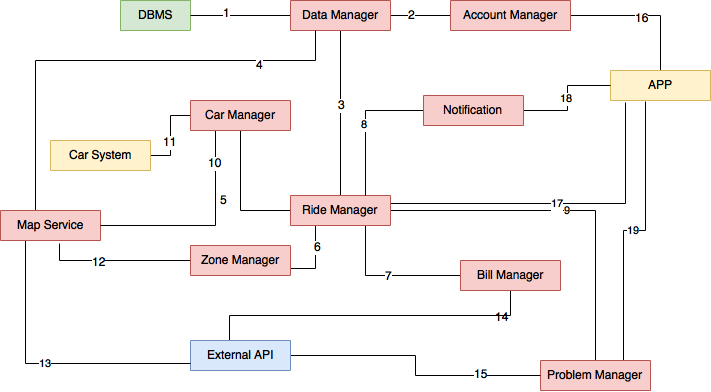
\includegraphics[width=\textwidth]{Diagrams/SoftwareIntegrationDiagram.png}
	\captionof{figure}{Software Integration Diagram}
	\label{Software Integration Diagram}
\end{center}

\subsection{Subsystem integration sequence}
The following diagram illustrates the integration sequence of the various subsystems, following the integration testing strategy described above. In particular, the Server Database is integrated before the Client, because the former does not need an actual functioning system in order to be tested efficiently, contrary to the latter.
%Image
\begin{center}
	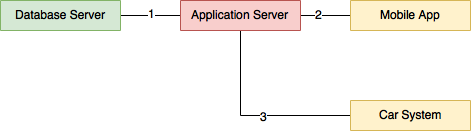
\includegraphics[width=\textwidth]{Diagrams/SubsystemsIntegrationDiagram.png}
	\captionof{figure}{Subsystem Integration Diagram}
	\label{Subsystem Integration Diagram}
\end{center}